\documentclass[10pt,a4paper]{article}
\usepackage[T1]{fontenc}
\usepackage{mathptmx}
\usepackage[scaled=0.90]{helvet}
\usepackage[margin=2.3cm]{geometry}
\usepackage{microtype}
\usepackage{amsmath,amssymb,amsthm,mathtools}
\usepackage{array,booktabs,tabularx,multirow,threeparttable}
\usepackage{graphicx}
\usepackage{tikz}
\usetikzlibrary{positioning,calc}
\usepackage{fancyvrb}
\usepackage[dvipsnames]{xcolor}
\usepackage{enumitem}
\usepackage[font=small,labelfont=bf]{caption}
\usepackage{subcaption}
\usepackage[authoryear,round]{natbib}
\usepackage[colorlinks=true,linkcolor=MidnightBlue,citecolor=MidnightBlue,urlcolor=MidnightBlue]{hyperref}
\usepackage[capitalise,noabbrev]{cleveref}
\hypersetup{pdftitle={Verdict Games and a Strategic View of the Turing Test},pdfauthor={Kaveh Aryan}}
\setlist{nosep,leftmargin=1.4em}
\setlength{\parskip}{0.25em}

\newtheorem{definition}{Definition}
\newtheorem{proposition}{Proposition}
\newtheorem{corollary}{Corollary}
\theoremstyle{remark}
\newtheorem{remark}{Remark}
\newtheorem{example}{Example}

\newcommand{\Cont}{\bot}
\newcommand{\E}{\mathbb{E}}
\newcommand{\G}{\mathsf{G}}
\newcommand{\I}{\mathsf{I}}
\newcommand{\adv}{\textsf{adv}}
\newcommand{\mini}{\textsf{min}}
\newcommand{\rnd}{\textsf{random}}
\newcommand{\intro}{\textsf{introspect}}
\newcommand{\look}{\textsf{lookahead}}
% generated by analysis/make_report.py -- do not edit
\newcommand{\AbstractFindings}{Under the conviction-seeking objective, one-step lookahead increased the primary judge's guilt score after four rounds of forced continuation by 2.3 points on a 0--100 scale (case-level 95\% CI 1.6--2.9) relative to baseline selection and exceeded introspective choice. It also raised scores for innocent defendants. Gains were smaller under held-out judges, and selection gains depended on the planner--evaluator pairing. Individual question-selection effects diminished under baseline continuation. A lookahead defence reduced guilt scores, but its selector queried an internal judge with access to withheld evidence. Under lookahead, a truth-seeking objective showed no clear discrimination improvement over the conviction-seeking objective. These findings concern score-guided policies within the specified simulator; their implications for human judgement and interactive AI detection remain to be tested.}
\newcommand{\AdvIntro}{+1.4 [+0.8, +2.1]}
\newcommand{\AdvIntroEst}{+1.4}
\newcommand{\AdvIntroP}{\ensuremath{<}0.001}
\newcommand{\AdvLook}{+2.3 [+1.6, +2.9]}
\newcommand{\AdvLookDefLook}{+2.2 [+1.3, +3.1]}
\newcommand{\AdvLookDefLookEst}{+2.2}
\newcommand{\AdvLookDefLookP}{\ensuremath{<}0.001}
\newcommand{\AdvLookDefRand}{+2.3 [+1.7, +3.0]}
\newcommand{\AdvLookDefRandEst}{+2.3}
\newcommand{\AdvLookDefRandP}{\ensuremath{<}0.001}
\newcommand{\AdvLookEst}{+2.3}
\newcommand{\AdvLookG}{+2.8 [+2.1, +3.6]}
\newcommand{\AdvLookGEst}{+2.8}
\newcommand{\AdvLookGP}{\ensuremath{<}0.001}
\newcommand{\AdvLookI}{+1.7 [+0.8, +2.6]}
\newcommand{\AdvLookIEst}{+1.7}
\newcommand{\AdvLookIP}{\ensuremath{<}0.001}
\newcommand{\AdvLookJudgeA}{+2.3 [+1.6, +2.9]}
\newcommand{\AdvLookJudgeAP}{\ensuremath{<}0.001}
\newcommand{\AdvLookJudgeB}{+0.6 [+0.1, +1.1]}
\newcommand{\AdvLookJudgeBP}{0.018}
\newcommand{\AdvLookJudgeC}{+1.5 [+0.4, +2.5]}
\newcommand{\AdvLookJudgeCP}{0.007}
\newcommand{\AdvLookJudgeD}{+1.0 [\ensuremath{-}0.3, +2.3]}
\newcommand{\AdvLookJudgeDP}{0.112}
\newcommand{\AdvLookJudgeE}{+1.4 [\ensuremath{-}0.5, +3.4]}
\newcommand{\AdvLookJudgeEP}{0.134}
\newcommand{\AdvLookJudgeF}{+0.8 [\ensuremath{-}0.9, +2.5]}
\newcommand{\AdvLookJudgeFP}{0.359}
\newcommand{\AdvLookP}{\ensuremath{<}0.001}
\newcommand{\AgreeDisc}{90}
\newcommand{\AgreeFab}{87}
\newcommand{\AgreeLead}{97}
\newcommand{\AuditAmbiguity}{4.14}
\newcommand{\AuditCoverContradicted}{5.00}
\newcommand{\AuditInnocentConsistent}{4.43}
\newcommand{\AuditStatementNeutral}{4.71}
\newcommand{\AuditWTrueBoth}{5.00}
\newcommand{\CRNShare}{77}
\newcommand{\CaseAuditPass}{56}
\newcommand{\CaseRegens}{2}
\newcommand{\CasesPositive}{42}
\newcommand{\CasesTotal}{48}
\newcommand{\ConvAdvLook}{+10.4 [+4.6, +16.2]}
\newcommand{\ConvAdvLookG}{+14.6 [+4.7, +24.5]}
\newcommand{\ConvAdvLookGEst}{+14.6}
\newcommand{\ConvAdvLookGP}{0.005}
\newcommand{\ConvAdvLookI}{+6.2 [\ensuremath{-}0.2, +12.7]}
\newcommand{\ConvAdvLookIEst}{+6.2}
\newcommand{\ConvAdvLookIP}{0.057}
\newcommand{\ConvDef}{\ensuremath{-}13.2 [\ensuremath{-}17.5, \ensuremath{-}8.9]}
\newcommand{\ConvDefEst}{\ensuremath{-}13.2}
\newcommand{\ConvDefP}{\ensuremath{<}0.001}
\newcommand{\ConvMinLook}{\ensuremath{-}1.0 [\ensuremath{-}6.8, +4.7]}
\newcommand{\ConvRateAll}{24.7}
\newcommand{\ConvRateG}{34.2}
\newcommand{\ConvRateI}{15.1}
\newcommand{\ConvThrAdvLookI}{+9.4 [+2.9, +15.8]}
\newcommand{\ConvThrAdvLookIEst}{+9.4}
\newcommand{\ConvThrAdvLookIP}{0.005}
\newcommand{\ConvType}{+19.1 [+12.8, +25.4]}
\newcommand{\ConvTypeEst}{+19.1}
\newcommand{\ConvTypeP}{\ensuremath{<}0.001}
\newcommand{\CrossAA}{0.86}
\newcommand{\CrossAE}{0.25}
\newcommand{\CrossEA}{0.30}
\newcommand{\CrossEE}{0.33}
\newcommand{\DeviationsText}{(1) Study 1 was restarted with more concurrent games, reusing cached responses where available. (2) 3 of 144 Study-2 decision points failed after retries (malformed candidate output) and were excluded under the stated failure rule. (3) Concurrent identical requests were not deduplicated. Identical first-round candidate lists were shared across all relevant cells in 77\% of case--objective groups; the two Study-2 planners also used separately realised hypothetical replies. These departures change the coupling between runs; variance reduction is not guaranteed. (4) The broad plan included exploratory utterance features, planner validity and split-sample selection. The implemented question coding, judge test--retest, TOST intervals and detailed Study-2 discrimination and validity analyses were added after the recorded freeze and are treated as exploratory.}
\newcommand{\DiscAdvIntr}{+3.8 [+2.9, +4.6]}
\newcommand{\DiscAdvIntrEst}{+3.8}
\newcommand{\DiscAdvIntrP}{\ensuremath{<}0.001}
\newcommand{\DiscAdvLook}{+3.5 [+2.7, +4.3]}
\newcommand{\DiscAdvLookEst}{+3.5}
\newcommand{\DiscAdvLookP}{\ensuremath{<}0.001}
\newcommand{\DiscAdvRand}{+2.4 [+1.5, +3.2]}
\newcommand{\DiscAdvRandEst}{+2.4}
\newcommand{\DiscAdvRandP}{\ensuremath{<}0.001}
\newcommand{\DiscBaseImmA}{\ensuremath{-}0.8 [\ensuremath{-}1.4, \ensuremath{-}0.2]}
\newcommand{\DiscBaseImmE}{+2.0 [+1.0, +2.9]}
\newcommand{\DiscChgAdvIntr}{+1.4 [+0.4, +2.4]}
\newcommand{\DiscChgAdvIntrEst}{+1.4}
\newcommand{\DiscChgAdvIntrP}{0.008}
\newcommand{\DiscChgAdvLook}{+1.1 [+0.1, +2.1]}
\newcommand{\DiscChgAdvLookEst}{+1.1}
\newcommand{\DiscChgAdvLookP}{0.029}
\newcommand{\DiscChgMinIntr}{+1.6 [+0.6, +2.6]}
\newcommand{\DiscChgMinIntrEst}{+1.6}
\newcommand{\DiscChgMinIntrP}{0.003}
\newcommand{\DiscChgMinLook}{+0.8 [\ensuremath{-}0.5, +2.1]}
\newcommand{\DiscChgMinLookEst}{+0.8}
\newcommand{\DiscChgMinLookP}{0.217}
\newcommand{\DiscMinIntr}{+3.9 [+3.1, +4.8]}
\newcommand{\DiscMinIntrEst}{+3.9}
\newcommand{\DiscMinIntrP}{\ensuremath{<}0.001}
\newcommand{\DiscMinLook}{+3.2 [+2.1, +4.3]}
\newcommand{\DiscMinLookEst}{+3.2}
\newcommand{\DiscMinLookP}{\ensuremath{<}0.001}
\newcommand{\DiscMinPickA}{+0.4 [\ensuremath{-}1.1, +1.9]}
\newcommand{\DiscMinPickE}{+0.7 [\ensuremath{-}1.4, +2.8]}
\newcommand{\DiscMinRand}{+2.4 [+1.6, +3.1]}
\newcommand{\DiscMinRandEst}{+2.4}
\newcommand{\DiscMinRandP}{\ensuremath{<}0.001}
\newcommand{\DiscROneAdvIntr}{+48 [+34, +62]}
\newcommand{\DiscROneAdvIntrP}{\ensuremath{<}0.001}
\newcommand{\DiscROneAdvLook}{+33 [+18, +49]}
\newcommand{\DiscROneAdvLookP}{\ensuremath{<}0.001}
\newcommand{\DiscROneMinIntr}{+45 [+29, +60]}
\newcommand{\DiscROneMinIntrP}{\ensuremath{<}0.001}
\newcommand{\DiscROneMinLook}{\ensuremath{-}4 [\ensuremath{-}26, +18]}
\newcommand{\DiscROneMinLookP}{0.705}
\newcommand{\DiscROneRandAdv}{42}
\newcommand{\DiscROneRandMin}{47}
\newcommand{\DiscSplitOracleA}{+2.3 [+0.7, +3.9]}
\newcommand{\DiscSplitOracleE}{\ensuremath{-}0.8 [\ensuremath{-}3.3, +1.7]}
\newcommand{\DriftAGFour}{77.5}
\newcommand{\DriftAGZero}{27}
\newcommand{\DriftAIFour}{74.3}
\newcommand{\DriftAIZero}{27}
\newcommand{\DriftEGFour}{71.1}
\newcommand{\DriftEGZero}{57}
\newcommand{\DriftEIFour}{62.2}
\newcommand{\DriftEIZero}{56}
\newcommand{\DriftFrom}{27}
\newcommand{\DriftTo}{76}
\newcommand{\FabAdv}{10}
\newcommand{\FabAdvLook}{+2.0 [\ensuremath{-}2.0, +5.9]}
\newcommand{\FabAdvLookP}{0.320}
\newcommand{\FabMin}{5}
\newcommand{\FabRoundFour}{14}
\newcommand{\FabRoundOne}{2}
\newcommand{\GLConv}{81}
\newcommand{\GLConvG}{90}
\newcommand{\GLConvI}{72}
\newcommand{\GLHOne}{+1.2 [+0.7, +1.6]}
\newcommand{\GLMean}{82.2}
\newcommand{\GLPAUC}{0.98}
\newcommand{\GLType}{+2.0 [+1.6, +2.3]}
\newcommand{\HEightFinal}{+0.22 [+0.00, +0.43]}
\newcommand{\HEightFinalP}{0.050}
\newcommand{\HEightImmediate}{+0.65 [+0.38, +0.92]}
\newcommand{\HEightImmediateP}{\ensuremath{<}0.001}
\newcommand{\HFiveCI}{\ensuremath{-}2.3 [\ensuremath{-}2.6, \ensuremath{-}2.0]}
\newcommand{\HFiveEst}{\ensuremath{-}2.3}
\newcommand{\HFiveP}{\ensuremath{<}0.001}
\newcommand{\HFivedz}{\ensuremath{-}2.15}
\newcommand{\HFourCI}{\ensuremath{-}0.3 [\ensuremath{-}1.7, +1.0]}
\newcommand{\HFourEst}{\ensuremath{-}0.3}
\newcommand{\HFourP}{0.624}
\newcommand{\HFourdz}{\ensuremath{-}0.07}
\newcommand{\HNineFinal}{+0.18 [+0.11, +0.25]}
\newcommand{\HNineFinalP}{\ensuremath{<}0.001}
\newcommand{\HNineImmediate}{+0.95 [+0.78, +1.13]}
\newcommand{\HNineImmediateP}{\ensuremath{<}0.001}
\newcommand{\HOneCI}{+2.3 [+1.6, +2.9]}
\newcommand{\HOneEst}{+2.3}
\newcommand{\HOneP}{\ensuremath{<}0.001}
\newcommand{\HOnedz}{+1.05}
\newcommand{\HSevenFinal}{+0.54 [+0.32, +0.75]}
\newcommand{\HSevenFinalP}{\ensuremath{<}0.001}
\newcommand{\HSevenImmediate}{+2.91 [+2.38, +3.45]}
\newcommand{\HSevenImmediateP}{\ensuremath{<}0.001}
\newcommand{\HSixCI}{+1.2 [+0.5, +1.9]}
\newcommand{\HSixEst}{+1.2}
\newcommand{\HSixP}{0.002}
\newcommand{\HSixdz}{+0.48}
\newcommand{\HThreeCI}{+1.7 [+0.8, +2.6]}
\newcommand{\HThreeEst}{+1.7}
\newcommand{\HThreeP}{\ensuremath{<}0.001}
\newcommand{\HThreedz}{+0.57}
\newcommand{\HTwoCI}{+0.8 [+0.3, +1.4]}
\newcommand{\HTwoEst}{+0.8}
\newcommand{\HTwoP}{0.005}
\newcommand{\HTwodz}{+0.42}
\newcommand{\HetPI}{[+0.0, +4.5]}
\newcommand{\HetTau}{1.1}
\newcommand{\HolmHEight}{\ensuremath{<}0.001}
\newcommand{\HolmHFive}{\ensuremath{<}0.001}
\newcommand{\HolmHFour}{0.624}
\newcommand{\HolmHNine}{\ensuremath{<}0.001}
\newcommand{\HolmHOne}{\ensuremath{<}0.001}
\newcommand{\HolmHSeven}{\ensuremath{<}0.001}
\newcommand{\HolmHSix}{0.005}
\newcommand{\HolmHThree}{\ensuremath{<}0.001}
\newcommand{\HolmHTwo}{0.010}
\newcommand{\KappaDisc}{0.80}
\newcommand{\KappaFab}{0.36}
\newcommand{\KappaLead}{0.00}
\newcommand{\MetaValue}{76.5}
\newcommand{\MinIntro}{+1.9 [+1.3, +2.6]}
\newcommand{\MinIntroEst}{+1.9}
\newcommand{\MinIntroP}{\ensuremath{<}0.001}
\newcommand{\MinLook}{+0.0 [\ensuremath{-}0.6, +0.6]}
\newcommand{\MinLookEst}{+0.0}
\newcommand{\MinLookG}{+0.4 [\ensuremath{-}0.4, +1.3]}
\newcommand{\MinLookGEst}{+0.4}
\newcommand{\MinLookGP}{0.325}
\newcommand{\MinLookI}{\ensuremath{-}0.4 [\ensuremath{-}1.3, +0.5]}
\newcommand{\MinLookIEst}{\ensuremath{-}0.4}
\newcommand{\MinLookIP}{0.420}
\newcommand{\MinLookP}{0.923}
\newcommand{\MinisterSignalText}{(in Study 2, the minister's simulated scores yielded +0.4 [\ensuremath{-}1.1, +1.9] points of discrimination gain, compared with +2.3 [+0.7, +3.9] for the split-sample selection benchmark)}
\newcommand{\NeutralConv}{25}
\newcommand{\ObjEffect}{\ensuremath{-}1.4 [\ensuremath{-}1.9, \ensuremath{-}0.9]}
\newcommand{\ObjEffectEst}{\ensuremath{-}1.4}
\newcommand{\ObjEffectP}{\ensuremath{<}0.001}
\newcommand{\PAUCAdvIntr}{0.94}
\newcommand{\PAUCAdvLook}{0.92}
\newcommand{\PAUCAdvRand}{0.83}
\newcommand{\PAUCMinIntr}{0.88}
\newcommand{\PAUCMinLook}{0.81}
\newcommand{\PAUCMinRand}{0.85}
\newcommand{\PAUCOverall}{98}
\newcommand{\PersistOneFin}{+0.46 [+0.10, +0.81]}
\newcommand{\PersistOneImm}{+4.29 [+3.39, +5.20]}
\newcommand{\PersistThreeFin}{+0.62 [+0.31, +0.92]}
\newcommand{\PersistThreeImm}{+1.54 [+1.19, +1.88]}
\newcommand{\PfinalMeanA}{75.9}
\newcommand{\PoneDriftFrom}{33}
\newcommand{\PoneDriftTo}{73}
\newcommand{\PoneTypeEst}{+0.5 [\ensuremath{-}1.1, +2.1]}
\newcommand{\ProviderText}{In Study 1, the player model was served by DeepInfra (67\%), Parasail (30\%), Venice (3\%) (all fp8). Launch order was randomised, but differing call counts and durations mean that provider fallback need not be balanced across conditions.}
\newcommand{\PtwoTypeEst}{+2.9 [+1.6, +4.2]}
\newcommand{\PxD}{\ensuremath{-}0.1 [\ensuremath{-}1.0, +0.8]}
\newcommand{\PxDEst}{\ensuremath{-}0.1}
\newcommand{\PxDP}{0.825}
\newcommand{\RateDisc}{55}
\newcommand{\RateFab}{8}
\newcommand{\RateLead}{97}
\newcommand{\RelFinalA}{0.07}
\newcommand{\RelFinalE}{0.04}
\newcommand{\RelImmediateA}{0.50}
\newcommand{\RelImmediateE}{0.19}
\newcommand{\RetestAMAD}{0.8}
\newcommand{\RetestAR}{0.99}
\newcommand{\RetestAVerdict}{98}
\newcommand{\RetestEMAD}{4.2}
\newcommand{\RetestER}{0.84}
\newcommand{\RetestEVerdict}{100}
\newcommand{\SelIntroFinal}{+0.56 [+0.31, +0.81]}
\newcommand{\SelIntroFinalP}{\ensuremath{<}0.001}
\newcommand{\SelIntroImmediate}{+2.03 [+1.45, +2.60]}
\newcommand{\SelIntroImmediateE}{+1.67 [+0.83, +2.51]}
\newcommand{\SelIntroImmediateP}{\ensuremath{<}0.001}
\newcommand{\SelLookAAdvOnEFinal}{+0.01 [\ensuremath{-}0.89, +0.91]}
\newcommand{\SelLookAAdvOnEFinalP}{0.984}
\newcommand{\SelLookAAdvOnEImmediate}{+1.31 [+0.45, +2.17]}
\newcommand{\SelLookAAdvOnEImmediateP}{0.004}
\newcommand{\SelLookAMinFinal}{+0.16 [\ensuremath{-}0.11, +0.42]}
\newcommand{\SelLookAMinFinalP}{0.235}
\newcommand{\SelLookAMinImmediate}{+0.16 [\ensuremath{-}0.51, +0.83]}
\newcommand{\SelLookAMinImmediateP}{0.630}
\newcommand{\SelLookEAdvOnAFinal}{+0.33 [+0.12, +0.53]}
\newcommand{\SelLookEAdvOnAFinalP}{0.002}
\newcommand{\SelLookEAdvOnAImmediate}{+1.00 [+0.46, +1.54]}
\newcommand{\SelLookEAdvOnAImmediateP}{\ensuremath{<}0.001}
\newcommand{\SelLookEAdvOnEFinal}{+0.55 [\ensuremath{-}0.01, +1.10]}
\newcommand{\SelLookEAdvOnEFinalP}{0.054}
\newcommand{\SelLookEAdvOnEImmediate}{+1.75 [+0.99, +2.51]}
\newcommand{\SelLookEAdvOnEImmediateP}{\ensuremath{<}0.001}
\newcommand{\SelOracleFinal}{+0.06 [\ensuremath{-}0.30, +0.43]}
\newcommand{\SelOracleFinalP}{0.735}
\newcommand{\SelOracleImmediate}{+2.97 [+2.46, +3.48]}
\newcommand{\SelOracleImmediateP}{\ensuremath{<}0.001}
\newcommand{\SoneNcases}{48}
\newcommand{\SoneNgames}{1,152}
\newcommand{\StudyTwoTransferText}{(H6). Study 2 also found an interaction between planner and evaluator on the standardised selection-gain scale (H8).}
\newcommand{\StwoNcont}{3,008}
\newcommand{\StwoNfail}{3}
\newcommand{\StwoNpoints}{141}
\newcommand{\TostHEight}{[+0.43, +0.87]}
\newcommand{\TostHFive}{[\ensuremath{-}2.51, \ensuremath{-}2.00]}
\newcommand{\TostHFour}{[\ensuremath{-}1.45, +0.79]}
\newcommand{\TostHNine}{[+0.81, +1.10]}
\newcommand{\TostHOne}{[+1.74, +2.79]}
\newcommand{\TostHSeven}{[+2.47, +3.36]}
\newcommand{\TostHSix}{[+0.60, +1.81]}
\newcommand{\TostHThree}{[+0.98, +2.42]}
\newcommand{\TostHTwo}{[+0.35, +1.29]}
\newcommand{\TotalCalls}{132,720}
\newcommand{\TotalCost}{20.62}
\newcommand{\TypeEffect}{+3.2 [+2.7, +3.6]}
\newcommand{\TypeEffectE}{+8.9 [+7.3, +10.5]}
\newcommand{\TypeEffectEst}{+3.2}
\newcommand{\TypeEffectP}{\ensuremath{<}0.001}
\newcommand{\ValImmAtoA}{0.52 [0.47, 0.57]}
\newcommand{\ValImmAtoE}{0.20 [0.14, 0.26]}
\newcommand{\ValImmEtoA}{0.17 [0.11, 0.23]}
\newcommand{\ValImmEtoE}{0.22 [0.16, 0.28]}


\title{\textbf{Verdict Games and a Strategic View of the Turing Test}}
\author{Kaveh Aryan\\King's College London\\\texttt{kaveh.aryan@kcl.ac.uk}}
\date{}

\begin{document}
\maketitle

\begin{abstract}
\noindent
\emph{Verdict games} model dialogues in which two speakers seek to influence a non-strategic judge that may end
the exchange with a binary decision. We define their information structure and payoffs, and establish conditions
under which stopped verdicts can be reconstructed from complete transcripts with the speakers' policies and internal
scoring models held fixed. We study these games using LLM prosecutors, defendants and judges in synthetic criminal
cases. A first experiment crosses prosecutor objectives, question-selection rules, defence rules and defendant types
across 48 cases, \SoneNgames{} games and six evaluators. Paired guilty and innocent versions of each case have identical
court evidence and different defendant briefs. A second experiment evaluates eight candidate questions at each sampled dialogue
state, using two continuations per question and defendant type. \AbstractFindings{}
\end{abstract}

% =====================================================================================================
\section{Introduction}

Language is not only a channel for communication but also an instrument of strategy. In a courtroom, the prosecution
and the defence exchange utterances whose purpose is to move a fact-finder; in an interrogation, the examiner chooses
questions to elicit statements that an impartial observer will find credible or damning; in a Turing test, a witness
produces language designed to avoid being classified as a machine \citep{oppy2021}. With large language models (LLMs)
now judged ``more human than humans'' in some settings \citep{rathi2024,jones2025} and increasingly used both as
conversational agents and as judges \citep{zheng2023}, the strategic structure of such dialogues has become a practical
question rather than a philosophical one.

We study \emph{verdict games}, in which two speakers influence a non-strategic judge through a sequence of exchanges.
The judge may stop after any exchange with one of two verdicts. The speakers can have different objectives: a
prosecutor may seek conviction regardless of guilt, whereas an examiner may seek a correct classification. These
objectives need not favour the same questions. A policy that increases convictions may improve discrimination between
guilty and innocent defendants, persuade the judge irrespective of truth, or exploit a particular evaluator's biases.

The model in \cref{sec:verdict} specifies the speakers' private information, the evidence available to the judge,
and the relation between verdicts and payoffs. A stopping-rule proposition gives conditions under which fixed
policies can be evaluated with several judges using the same transcripts. It does not assume that the speakers would
retain those policies if they were informed of a change in judge.

We investigate strategic question selection in two experiments with LLM prosecutors, defendants and judges.
Study 1 crosses two prosecutor objectives, three prosecutor selection rules, two defence rules and two defendant
types across 48 cases (\cref{sec:study1}). The selection rules share a candidate-generation protocol, allowing us
to compare choosing without evaluation, introspective choice and explicit simulation of a reply. Matched guilty and
innocent defendants distinguish changes in perceived guilt from changes in discrimination. Study 2 branches each
sampled dialogue state into all eight proposed questions and runs two continuations per question and defendant type
(\cref{sec:study2}). It examines the immediate effect of selection, its persistence, and its dependence on the
planner's internal judge. These experiments estimate effects within the specified simulator; inference to other
cases, models or human interactions requires additional assumptions (\cref{sec:causal}).

% =====================================================================================================
\section{Verdict Games}\label{sec:verdict}

\subsection{Definition and examples}
\begin{definition}[Verdict game]\label{def:verdict}
A verdict game is a finite-horizon extensive-form game with two speakers, $X$ (the examiner) and $Y$ (the respondent),
and a non-strategic classifier $C$. Fix a public context $s_0$, finite type spaces $T_X,T_Y$ with common prior
$\mu(\cdot\mid s_0)$, a finite alphabet $\Sigma$, an utterance-length bound $l$ and a horizon $d$.
Each speaker observes its own type. At stage $k=1,\dots,d$, $X$ appends an utterance $v_k$ and then $Y$ appends
$w_k$, with $|v_k|,|w_k|\le l$, producing $h_k=(v_1,w_1,\dots,v_k,w_k)$. The judge observes
$\omega=(s_0,\pi_C(t_X,t_Y))$ and the transcript, where $\pi_C$ specifies the disclosed private information.
In the deterministic case, the classifier is
\begin{equation}
C:\ \Omega\times H\ \to\ \{0,1,\Cont\}
\end{equation}
where $H$ is the set of admissible transcript prefixes and $\Omega$ the space of judge information.
After each exchange it returns $c_k=C(\omega,h_k)$, where $\Cont$ means ``continue''. The game stops at the first $k\le d$ for which
$c_k\ne\Cont$, with that verdict as its outcome; if no such stage exists, its outcome is $\Cont$ at $d$.
Speaker $i$ receives $u_i(t_X,t_Y,c)$. A behavioural strategy maps that speaker's information history to a
distribution over utterances. Without additional signals these histories are $(t_X,s_0,h_{k-1})$ for $X$ and
$(t_Y,s_0,h_{k-1},v_k)$ for $Y$. If a policy can query an internal scoring oracle, the permitted queries, the
oracle's information and its returned scores are also specified as part of the information structure; the strategy
may condition on those scores. The stopping classifier may be randomised, using exogenous random draws and
information available at the current stage.
\end{definition}

The judge may see evidence that one speaker does not. In the experiments, the prosecution and judge receive
withheld records, while the defendant initially receives only the public file and its private account.

\begin{example}[Court game]
$X$ is the prosecution, $Y$ the defence, $c=1$ is ``guilty'' and $c=0$ ``not guilty''. Payoffs depend only on the
verdict: $u_X(1)=1$ and $u_X(0)=u_X(\Cont)=-1$, the last equality expressing the presumption of
innocence, and $u_Y=-u_X$. The game is zero-sum, although the speakers may hold private information.
\end{example}

\begin{example}[Interrogation game]\label{ex:interrog}
$T_Y=\{\G,\I\}$ (guilty, innocent). The examiner is rewarded for a correct decisive verdict and penalised for a wrong one:
$u_X(\G,1)=u_X(\I,0)=1$, $u_X(\G,0)=u_X(\I,1)=-1$ and $u_X(\cdot,\Cont)=0$; both types of $Y$ seek exoneration:
$u_Y(t_Y,0)=u_Y(t_Y,\Cont)=1$ and $u_Y(t_Y,1)=-1$. For the examiner this is the usual unweighted classification
utility; unequal costs of the two classification errors can be represented by different payoffs.
\end{example}

\begin{example}[Turing test]\label{ex:turing}
Relabelling $\G,\I$ as \emph{machine}, \emph{human} gives the Turing test as an interrogation game, with $C$ an
AI-detection procedure that may decide after any exchange. Viewing the test as a game makes two things explicit: the
witness's best response is to minimise detectability rather than to display intelligence, and the detector's power
depends on the questions it is shown. Static detectors of machine text \citep{mitchell2023,mireshghallah2024} were not
built for adversarially produced dialogue; an interactive, strategic interrogator---a Voight-Kampff test---is the
natural counterpart. The experiments below use this payoff distinction in a criminal-case simulation, with guilt
in the role of machine identity.
\end{example}

\begin{figure}[t]
\centering
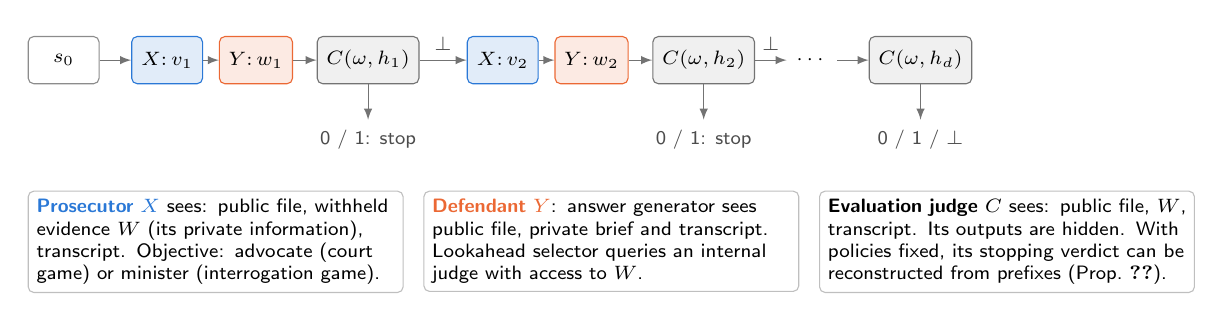
\begin{tikzpicture}[
  font=\sffamily\scriptsize, >=latex,
  st/.style={draw=black!45, rounded corners=2pt, minimum height=6mm, minimum width=9mm, fill=white, line width=0.4pt},
  xm/.style={st, fill=xblue!14, draw=xblue},
  ym/.style={st, fill=yorange!14, draw=yorange},
  jm/.style={st, fill=black!6, draw=black!55, minimum width=11mm},
  view/.style={draw=black!25, rounded corners=2pt, align=left, inner sep=3pt, text width=4.55cm, line width=0.4pt}]
\definecolor{xblue}{HTML}{2a78d6}\definecolor{yorange}{HTML}{eb6834}
\node[st] (s0) at (0,0) {$s_0$};
\node[xm, right=4mm of s0] (v1) {$X{:}\,v_1$};
\node[ym, right=2mm of v1] (w1) {$Y{:}\,w_1$};
\node[jm, right=3mm of w1] (c1) {$C(\omega,h_1)$};
\node[xm, right=6mm of c1] (v2) {$X{:}\,v_2$};
\node[ym, right=2mm of v2] (w2) {$Y{:}\,w_2$};
\node[jm, right=3mm of w2] (c2) {$C(\omega,h_2)$};
\node[right=4mm of c2] (dots) {$\cdots$};
\node[jm, right=4mm of dots] (cd) {$C(\omega,h_d)$};
\draw[->, black!55] (s0) -- (v1); \draw[->, black!55] (v1) -- (w1); \draw[->, black!55] (w1) -- (c1);
\draw[->, black!55] (c1) -- node[above, black!70]{$\bot$} (v2); \draw[->, black!55] (v2) -- (w2); \draw[->, black!55] (w2) -- (c2);
\draw[->, black!55] (c2) -- node[above, black!70]{$\bot$} (dots); \draw[->, black!55] (dots) -- (cd);
\draw[->, black!55] (c1.south) -- ++(0,-0.45) node[below, black!70]{0 / 1: stop};
\draw[->, black!55] (c2.south) -- ++(0,-0.45) node[below, black!70]{0 / 1: stop};
\draw[->, black!55] (cd.south) -- ++(0,-0.45) node[below, black!70]{0 / 1 / $\bot$};
\node[view, anchor=north west] (vx) at ($(s0.south west)+(0,-1.35)$) {\textbf{\color{xblue}Prosecutor $X$} sees: public file, withheld evidence $W$ (its private information), transcript. Objective: advocate (court game) or minister (interrogation game).};
\node[view, anchor=north west] (vy) at ($(vx.north east)+(0.25,0)$) {\textbf{\color{yorange}Defendant $Y$}: answer generator sees public file, private brief and transcript. Lookahead selector queries an internal judge with access to $W$.};
\node[view, anchor=north west] (vc) at ($(vy.north east)+(0.25,0)$) {\textbf{Evaluation judge $C$} sees: public file, $W$, transcript. Its outputs are hidden. With policies fixed, its stopping verdict can be reconstructed from prefixes (Prop.~\ref{prop:decouple}).};
\end{tikzpicture}
\caption{A verdict game with the information structure used in the experiments. Each stage consists of a question
from $X$ and an answer from $Y$; the classifier then stops the game with a verdict or lets it continue ($\bot$), up to
$d$ stages. Guilty and innocent versions of a case share the public file and the withheld evidence and differ only in
$Y$'s private brief.}
\label{fig:game}
\end{figure}


\subsection{Strategic policies}\label{sec:policies}
Utterance spaces are astronomically large, so exact equilibrium computation is out of reach. We study instead families
of policies built around a \emph{generator} $g(\cdot\mid\text{view},h)$, an LLM prompted with the player's objective
and view of the game. For $K\ge1$, let $V_K=(v^{(1)},\dots,v^{(K)})$ be $K$ candidates proposed by $g$.
\begin{itemize}
  \item \textbf{Random}: select a candidate without evaluating its content. The implementation uses a reproducible
  hash of the generation-request key to choose an index in $V_K$; this is the baseline selection policy.
  \item \textbf{Introspect}: the same LLM, shown $V_K$ in a randomised order, picks the candidate that ``best serves
  your goal'', with no explicit simulation.
  \item \textbf{Lookahead}: a one-step selection heuristic using an internal respondent model and a surrogate
  score from a model of the judge. Let $\hat Y_t$ simulate a type-$t$ respondent using the public file and transcript,
  without the actual defendant's private brief or undisclosed evidence. With
  $\hat p(\cdot)\in[0,1]$ the internal judge's guilt score and fixed weights $\hat\mu(\G)=\hat\mu(\I)=1/2$,
  \begin{equation}\label{eq:lookahead}
  v^\star\in\arg\max_{v\in V_K}\ \sum_{t\in T_Y}\hat\mu(t)\ \E_{w\sim\hat Y_t(\cdot\mid h,v)}\Big[\tilde u_X\big(t,\hat p(\omega,h\,v\,w)\big)\Big],
  \end{equation}
  where $\tilde u_X(t,p)=p$ for the court (advocate) objective and $\tilde u_X(\G,p)=p$, $\tilde u_X(\I,p)=1-p$ for
  the interrogation (minister-of-justice) objective. The respondent's lookahead chooses
  $w^\star\in\arg\min_{w\in W_K}\hat p(\omega,h\,v\,w)$.
\end{itemize}
The expectation in \cref{eq:lookahead} is approximated by one simulated reply per type. The fixed type weights
are not updated from the transcript, and the next-stage guilt score is a surrogate for the terminal verdict payoff.
Thus the rule is not an exact Bayesian best response in the verdict game. Candidate generation is held fixed
within an objective, but introspection and lookahead use additional model calls; total inference cost is not matched.

\subsection{Evaluating judges on fixed transcripts}
The evaluation judge does not generate either player's utterances. This permits the simulation to finish a dialogue
and subsequently determine where a given judge would have stopped it, subject to the following invariance condition.

\begin{proposition}[Reconstruction of stopped outcomes]\label{prop:decouple}
Fix the context, type distribution and policy kernels at every history, including any internal judge used for
planning. Suppose these kernels are the same whether play is stopped by $C$ or continued to $d$: players receive
no outputs from the external stopping evaluation or stopping-regime indicator, and their policies are not adapted
to a replacement evaluator.
Let $\tilde h_d$ be a dialogue generated by these policies without stopping. Apply the non-anticipating classifier
$C$ to successive prefixes and return its first decisive verdict, or $\Cont$ if none occurs by $d$; denote this
operation by $\Phi_C(\omega,\tilde h_d)$. For a randomised classifier, preserve the joint response law of
internal scoring and external evaluation, including any shared randomness. Then $\Phi_C$ has the same distribution as the outcome of the stopped
game under the fixed policies and $C$.
\end{proposition}
\begin{proof}
Couple the two executions using the same types, internal-oracle responses, utterance draws and classifier draws.
Their initial histories agree.
If they agree through stage $k-1$ and the stopped game remains active, the invariant policy kernels produce the same
two utterances at stage $k$. The classifier then receives the same prefix and, with the coupled draw, returns the
same output. Induction gives identical prefixes through the first decisive verdict, so both procedures stop at the
same stage with the same outcome. If neither has a decisive verdict, both return $\Cont$ at $d$.
\end{proof}

\begin{corollary}
For a fixed pair of policies satisfying the proposition, several classifiers can be evaluated on the same complete
transcripts. Each gives the stopped-outcome distribution for that evaluator with the policies held fixed. This
comparison does not describe how players would adapt to a new judge or an equilibrium under that judge.
\end{corollary}
\noindent For example, if a judge first returns a decisive verdict at round~2, later rounds are discarded when
computing that judge's verdict-game outcome. Its probability of guilt at round~4 is a different quantity: an
assessment under forced continuation, which is the primary Study-1 outcome. Hidden outputs alone are insufficient
if players change their behaviour because they know the judge or infer information from survival; the proposition
requires the policy kernels to remain fixed. Our simulation uses fixed prompts and supplies neither judge feedback
nor a separate survival signal. A stochastic judge still introduces evaluation uncertainty.

\subsection{Equilibrium and meta-games}
Bounded utterances and a finite horizon give a finite dialogue tree. Even when court-game
payoffs do not depend on guilt, private evidence and briefs can create imperfect information; ordinary backward
induction therefore does not generally apply. Bayesian or sequential equilibrium concepts account for these
information sets \citep{tadelis2013}. We instead use empirical game-theoretic analysis \citep{wellman2006},
restricting each player to the tested policies. The reported zero-sum meta-game uses mean final probability of guilt
as its payoff surrogate, rather than the first decisive verdict. Its equilibrium describes the estimated policy
matrix, not an equilibrium of the unrestricted verdict game.

% =====================================================================================================
\section{Experimental Design and Statistical Analysis}\label{sec:causal}

\paragraph{Units and interventions.}
A case $c$ consists of a public file, withheld evidence and two private briefs. A policy profile
$z=(o,a,b)$ specifies the prosecutor's objective $o\in\{\adv,\mini\}$, its selection rule
$a\in\{\rnd,\intro,\look\}$ and the defence rule $b\in\{\rnd,\look\}$. Defendant type
$t\in\{\G,\I\}$ is a within-case factor: the court file is identical and only the private brief changes.
Let $Y^e_c(z,t)$ be evaluator $e$'s guilt score after $d$ rounds of forced continuation under $(z,t)$, and
$\mu^e_c(z,t)=\E[Y^e_c(z,t)\mid c]$. The expectation includes randomness in generation, selection and evaluation.
This fixed-horizon score is distinct from the first-decisive-verdict outcome reconstructed by
\cref{prop:decouple}.

\paragraph{Policy effects.}
For two profiles, define the case-specific contrast
\begin{equation}
\tau^e_c(z,z')=\tfrac12\sum_{t\in\{\G,\I\}}\bigl[\mu^e_c(z,t)-\mu^e_c(z',t)\bigr],
\qquad
\tau^e_{\mathcal C}(z,z')=\frac1n\sum_{c\in\mathcal C}\tau^e_c(z,z'),
\end{equation}
where $\mathcal C$ is the analysed case bank. The \emph{strategic advantage} compares
$(\adv,\look,b)$ with $(\adv,\rnd,b)$ and averages over defence rules $b$. Discrimination is
$\Delta^e_{\mathcal C}(z)=n^{-1}\sum_c[\mu^e_c(z,\G)-\mu^e_c(z,\I)]$.
We also report paired AUC: within each case and defendant type, scores are first averaged over the factors not
specified in the comparison; we then count the proportion of cases with a higher guilty than innocent mean,
with ties counting as one half. This quantity depends on the averaging and coupling of the underlying runs.
An increase in perceived guilt for both types need not improve discrimination. The \emph{transfer gap} compares a
policy contrast under the planner's internal judge with the same contrast under held-out evaluators.

\paragraph{Identification within the simulator.}
Copies of a case can be run under each policy profile, providing samples from each intervention's outcome
distribution \citep{holland1986,imbens2015}. The causal interpretation requires well-specified interventions,
stable response laws, and no effect of another case's treatment on the outcome distribution of the current case.
These are the consistency and no-interference requirements commonly grouped under SUTVA; stateless prompts support
them but do not establish them for a hosted service with shared routing, caches and resource limits. Complete
crossing provides observations for every Study-1 cell, so comparisons need no extrapolation across unobserved
policy profiles. Missing or failed runs require separate consideration: a stated exclusion rule alone does not
make failures independent of outcomes.

Under these conditions, a within-case contrast $D_c$ of observed scores satisfies
$\E[D_c\mid c]=\tau^e_c$, and $\hat\tau=n^{-1}\sum_cD_c$ is unbiased for the mean effect over the fixed case bank.
Sampling every condition does not reveal its expected outcome exactly. Repeated runs reduce Monte Carlo uncertainty
within the simulator; they do not remove uncertainty about the choice of cases, the simulator's assumptions or its
relevance to human behaviour. For Study 2, the reported averages concern the completed decision points; extending
those estimates to the three failed points requires an assumption about the failure mechanism.

\paragraph{Case-level inference.}
A population target $\tau^e_{\mathcal P}=\E_{c\sim\mathcal P}[\tau^e_c]$ additionally requires a sampling model for
cases. Under such a model, the law of total variance gives
\begin{equation}
\operatorname{Var}(D_c)=\operatorname{Var}_c(\tau^e_c)+
\E_c[\operatorname{Var}(D_c\mid c)].
\end{equation}
The second term includes covariance between coupled runs of the same case. Our $t$-intervals and case bootstrap
use cases as the independent clusters and reflect both observed between-case variation and simulation variation.
The 48 cases are balanced, generated and audited stimuli, not a probability sample of criminal cases; population
interpretations of these intervals rely on treating them as exchangeable examples from a comparable synthetic
case-generation process. More repetitions of a single case cannot establish generality across cases
\citep{judd2012,westfall2014}. Within-case comparisons cancel an additive common case effect, but not
case-by-treatment interactions or every possible benefit of covariate adjustment.

\paragraph{Shared draws and service variation.}
Models, prompts, decoding parameters and selection rules specify the intended interventions. A shared cache reuses
responses for matching requests and sample indices, coupling some draws across conditions. For two scores $A,B$,
$\operatorname{Var}(A-B)=\operatorname{Var}(A)+\operatorname{Var}(B)-2\operatorname{Cov}(A,B)$: common random
numbers reduce contrast variance when the induced covariance is positive \citep{law2015}. Reuse alone does not
guarantee that sign. Concurrent duplicate requests were not deduplicated, and only \CRNShare\% of the
case--objective groups shared identical first-round candidate lists across all their cells. Study 1 randomised game
launch order to reduce systematic temporal confounding. Different call counts, durations and provider fallbacks
can nevertheless produce condition-dependent service histories; randomised launch order does not guarantee
provider balance. Recorded transcripts and judgements, rather than a fresh replay, define the analysed data.

% =====================================================================================================
\section{Materials, Agents and Judges}\label{sec:materials}

\paragraph{Cases.} The stimulus bank contains 56 synthetic criminal cases (8 for stimulus validation, 48 for the main experiments), generated from a balanced
design over 14 charges, 4 settings, 3 levels of designed evidence strength and defendant gender (16 main cases per
strength level). Following the Strategic Use of Evidence paradigm from interviewing research \citep{hartwig2006}, each
case has four public evidence items, a vague initial statement, and two \emph{withheld} items: records of the
defendant's own movements or contacts (card transactions, phone-cell data, entry logs) that the prosecution and the
judge see but the defendant's answer generator does not initially receive. The withheld facts are true in both worlds. In the guilty world they are part of
the crime, and the defendant's prepared cover story denies or misstates them; in the innocent world they have ordinary
reasons that the defendant would readily admit. Innocent defendants also carry an unrelated embarrassing secret, so that
evasiveness alone is not diagnostic. Cases were audited by an LLM against five criteria (ambiguity of the public evidence,
withheld facts true in both worlds, cover story contradicted, innocent account consistent, neutral initial statement).
A first generator (GPT-4.1-mini) failed the audit for most cases, typically by making withheld items forensic proof of
the crime rather than neutral records, so we discarded its output and regenerated every case with Claude Haiku 5.5
(with reasoning). Audited by DeepSeek-V4-Flash, \CaseAuditPass{} of 56 cases passed, \CaseRegens{} after one
regeneration (scores in \cref{app:cases}). In Study 1 the guilty twin was judged
guiltier than the innocent twin in \PAUCOverall\% of cases. Defendants' names were reassigned from a diverse,
gender-matched list after the generator repeatedly selected a few names. Names are held constant across a case's
conditions, although their interaction with a treatment is not separately estimated.

\paragraph{Agents.} All players and the planners' simulators are Qwen3-235B-A22B-Instruct-2507 (fp8, served mainly by
DeepInfra with logged fallback to other fp8 providers; temperature 1). The prosecutor sees the public file, the withheld evidence and the transcript, and decides whether and
when to reveal what it holds; the defendant's answer generator sees the public file, its private brief and the transcript. Each round the
prosecutor's generator proposes $K=4$ questions ($\le$50 words), the defendant's proposes $K=4$ answers (40--80
words), and the selection rules of \cref{sec:policies} choose among them; utterances are capped at $l=80$ words and
games last $d=4$ rounds. The lookahead planner scores each candidate question by simulating one hypothetical guilty and
one hypothetical innocent reply and querying its internal judge on both; the defence's lookahead queries the internal
judge on each candidate answer. That internal judge receives the full court file, including withheld evidence.
Consequently the defence selector has access to an evidence-informed scoring oracle even though its answer generator
does not see the withheld records. Its advantage measures the effect of this implemented selection procedure,
including that scoring access. The internal scoring model is held fixed when transcripts are evaluated by other
judges. Prompts are reproduced in \cref{app:prompts}.

\paragraph{Judges.} After every round the judge reads the court's file and the transcript and returns a probability of
guilt and a verdict label (\textsc{guilty} beyond reasonable doubt, \textsc{not guilty}, or \textsc{continue}), at
temperature 0. The primary judge, which is also the planner's internal judge in Study~1, is GPT-4o-mini. For GPT-4o-mini and Llama, we request up to 20 token log probabilities at each output position. At the first
integer-token position, we take the probability-weighted mean of the returned integer tokens in 0--100,
renormalising their available mass. If that mass is below 0.5 or unavailable, we use the stated probability.
This \emph{soft} score follows the token-weighting approach of G-Eval \citep{liu2023geval}, but is a truncated-token
summary, not the mean of the full distribution. It reduces ties relative to the often coarsely rounded stated
probabilities; it does not establish calibration. Five held-out judges---Llama-3.3-70B (soft),
Gemini-2.5-Flash-Lite, Claude-Haiku-5.5, DeepSeek-V4-Flash and Mistral-Small-3.2 (stated probabilities)---evaluate the
same transcripts post hoc (\cref{prop:decouple}). The verdict-game outcome is the first decisive label over rounds
1--4, with \textsc{continue} at round 4 counting as acquittal.

\paragraph{Implementation.} Calls go through OpenRouter with preferred providers, permitted fallbacks and the serving provider logged per call;
responses are cached under a hash of their inputs; the run order of games is randomised; and a hard budget guard
stopped spending at the pre-set limit. All calls, including stimulus validation, cost
\TotalCost{}~USD (\cref{app:repro}).

% =====================================================================================================
\section{Stimulus Validation}\label{sec:validation}

An initial experiment used eight validation cases without withheld evidence and crossed all 24 conditions
(192 games). The estimated guilty--innocent score difference was \PoneTypeEst{} points, while the primary
judge's probability of guilt rose from \PoneDriftFrom{} before examination to \PoneDriftTo{} after four rounds.
Thus the initial setup provided little evidence that the dialogue distinguished the two defendant types.
This motivated cases with verifiable withheld records (\cref{sec:materials}) and longer answers; the initial
answers had averaged about 23 words.

A second validation experiment used the same eight cases with the revised evidence structure (192 games).
The guilty--innocent difference was \PtwoTypeEst{}, and the variation of within-case contrasts informed the
sample-size calculations. The hypotheses and analysis code were then recorded in an internal pre-registration
before the main runs, according to the timestamp in the accompanying files (\cref{app:prereg};
\citealp{nosek2018}). These validation observations are analysed separately from the 48 main cases.

% =====================================================================================================
\section{Study 1: Strategic Play and Discrimination}\label{sec:study1}

\subsection{Design}
Study 1 is a complete randomised-block design with case as the block. Every one of the 48 main cases is played under all
$2\times3\times2\times2=24$ combinations of the prosecutor's objective (advocate, minister), the prosecutor's selection
rule (random, introspect, lookahead), the defence's selection rule (random, lookahead) and the defendant's type
(guilty, innocent), one game per cell, for \SoneNgames{} games in randomised run order. The design compares complete policy procedures. Within an objective, the rules use the same candidate-generation
protocol: lookahead versus random selection measures the effect of evaluating candidates by simulated replies,
and lookahead versus introspection compares explicit simulation with the model's direct choice. These contrasts
include the additional inference used by each selector. The objective factor changes both the prosecutor's goal
instruction and the lookahead utility, so its effect is not attributable to the utility formula alone. Crossing
these factors with defendant type measures discrimination, while the defence factor tests the effect of a
countervailing selection policy with the scoring access described in \cref{sec:materials}.

\paragraph{Hypotheses and analysis.} The specified hypotheses H1--H6 and their contrasts are listed in
\cref{tab:confirm}; the primary outcome is the primary judge's soft probability of guilt after round~4 (0--100). Each
contrast is computed within case (averaging over the factors it does not name) and tested across the 48 cases with a
two-sided $t$-test, with Holm correction over the nine confirmatory hypotheses of both studies. Bootstrap and sign-flip
results are in \cref{app:prereg}. The second validation experiment supplied the variance estimates for power calculations: with 48 cases the minimum detectable effect at 80\% power
is about 1.3 points for H1 and H3, 0.5 points for H5 and 0.8 points for H2, while H4 was expected to be underpowered.

\subsection{Results}

\paragraph{Manipulation and measurement checks.}
The recorded conversations distinguished defendant types on average. Under the primary judge,
guilty twins ended \TypeEffect{} points above their innocent twins, and in \PAUCOverall\% of cases the guilty twin
was judged guiltier (averaging over the 12 cells). The verdict-game rule convicted \ConvRateG\% of guilty and
\ConvRateI\% of innocent defendants. All six judges discriminated in the same direction (\cref{tab:judges}); DeepSeek
did so most strongly (\TypeEffectE{}). Both judges evaluated at every round showed \emph{examination drift}
(\cref{fig:drift}): the primary judge's probability of guilt rose from \DriftAGZero{} before the examination to
\DriftAGFour{} (guilty) and \DriftAIFour{} (innocent) after four rounds, as in the validation experiments. This pattern is consistent with an incriminating effect of
continued examination, but the design does not isolate question count from the content of the exchanges. The primary judge is
close to deterministic: re-querying 200 random prefixes gave $r=\RetestAR$ with a mean absolute difference of
\RetestAMAD{} points and \RetestAVerdict\% verdict agreement. DeepSeek, which reports stated probabilities, was
noisier ($r=\RetestER$, \RetestEMAD{} points).

\begin{table}[t]
\centering\small
\caption{Confirmatory hypothesis tests (Study 1: H1--H6, outcome = primary judge's probability of guilt after
round 4, in points; Study 2: H7--H9, immediate outcome). Estimates are means of within-case contrasts over 48 cases;
$d_z$ is the mean divided by the SD of case-level contrasts; $p_{\text{Holm}}$ adjusts across all nine hypotheses.}
\label{tab:confirm}
\begin{tabular}{@{}llrlrrr@{}}\toprule
 & Contrast & Estimate & 95\% CI & $d_z$ & $p$ & $p_{\text{Holm}}$\\\midrule
H1 & Strategic advantage: advocate lookahead $-$ random & +2.27 & [+1.64, +2.89] & +1.05 & \ensuremath{<}0.001 & \ensuremath{<}0.001\\
H2 & Simulation vs introspection (advocate) & +0.82 & [+0.26, +1.39] & +0.42 & 0.005 & 0.010\\
H3 & Advocate lookahead $-$ random, innocent defendants & +1.70 & [+0.84, +2.56] & +0.57 & \ensuremath{<}0.001 & \ensuremath{<}0.001\\
H4 & Discrimination: minister $-$ advocate (lookahead) & \ensuremath{-}0.33 & [\ensuremath{-}1.68, +1.01] & \ensuremath{-}0.07 & 0.624 & 0.624\\
H5 & Defence lookahead $-$ random & \ensuremath{-}2.26 & [\ensuremath{-}2.57, \ensuremath{-}1.95] & \ensuremath{-}2.15 & \ensuremath{<}0.001 & \ensuremath{<}0.001\\
H6 & Transfer gap: planner's judge $-$ held-out judges & +1.20 & [+0.48, +1.93] & +0.48 & 0.002 & 0.005\\
H7 & Move value: planner pick $-$ random (immediate) & +2.91 & [+2.38, +3.45] & +1.59 & \ensuremath{<}0.001 & \ensuremath{<}0.001\\
H8 & Crossover: matched $-$ mismatched (SD units) & +0.65 & [+0.38, +0.92] & +0.71 & \ensuremath{<}0.001 & \ensuremath{<}0.001\\
H9 & Dose-response slope per doubling of $k$ & +0.95 & [+0.78, +1.13] & +1.57 & \ensuremath{<}0.001 & \ensuremath{<}0.001\\
\bottomrule\end{tabular}

\end{table}

\paragraph{Confirmatory tests.}
\Cref{tab:confirm} reports the nine specified tests. Lookahead raised the advocate's probability of guilt by
\HOneCI{} points (H1, $d_z={}$\HOnedz, $p_{\text{Holm}}$\,\HolmHOne). This is a large and consistent standardised effect, but modest in absolute terms. In verdict terms it adds
\ConvAdvLook{} percentage points to the conviction rate. Explicit simulation exceeded introspective choice under
the same candidate-generation protocol by \HTwoCI{}
(H2), so modelling the opponent and the judge adds value beyond the LLM's unaided judgement. Lookahead raised the
probability of guilt for \emph{innocent} defendants by \HThreeCI{} (H3). There was no clear difference in discrimination
between minister and advocate objectives under lookahead (H4: \HFourCI{}; the 90\% interval \TostHFour{} contains zero but also effects of more than one point
in favour of the advocate, so this is an inconclusive null rather than evidence of equivalence). A lookahead defence
changed the probability of guilt by \HFiveCI{} (H5, $d_z={}$\HFivedz). The strategic advantage was \HSixCI{} points larger
when measured by the judge the planner had modelled than when averaged over the five held-out judges (H6).

\begin{figure}[t]
\centering
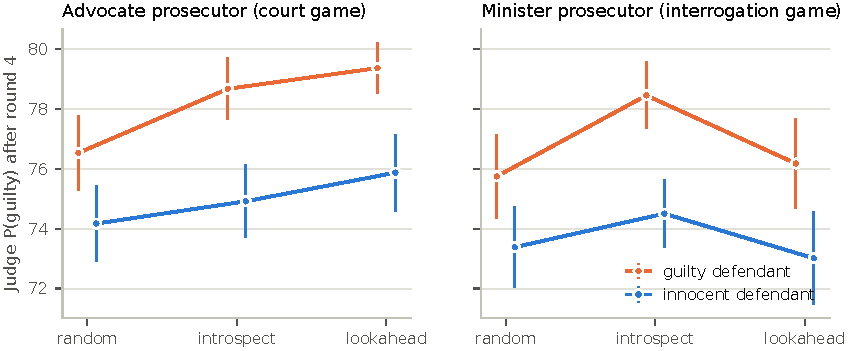
\includegraphics[width=\linewidth]{figs/s1_cells.pdf}
\caption{Study 1: primary judge's probability of guilt after round 4 by prosecutor objective, selection rule and
defendant type, averaged over the defence factor. Error bars are 95\% intervals of cell means across the 48 cases. These intervals describe cell means; uncertainty in a paired contrast also depends on covariance between cells
and should be read from \cref{tab:confirm}.}
\label{fig:cells}
\end{figure}

\paragraph{Discrimination and conviction.}
\Cref{fig:cells} decomposes the effect by defendant type. For the advocate, lookahead raised the probability of guilt
for guilty defendants by \AdvLookG{} and for innocent defendants by \AdvLookI{}, so it improved discrimination by
\DiscChgAdvLook{} points: strategy here is partly informative. In verdict terms, it raised convictions of guilty
defendants by \ConvAdvLookG{} percentage points and of innocent defendants by \ConvAdvLookI{} ($p=\ConvAdvLookIP$).
Under the post hoc threshold classifier ($P\ge80$), wrongful convictions rose by \ConvThrAdvLookI{} points
($p=\ConvThrAdvLookIP$). The court-game objective therefore buys more correct convictions at the price of more
wrongful ones, which is exactly the trade-off a strategic interrogator in a Turing test would face between catching
machines and flagging humans. Under the minister objective, the estimated lookahead effect was small and uncertain (\MinLook{}). It did not, however, buy better truth-tracking: the minister's discrimination
change under lookahead was \DiscChgMinLook{}. The arm that improved discrimination most reliably was introspection, by
\DiscChgAdvIntr{} (advocate) and \DiscChgMinIntr{} (minister) points.

\paragraph{Evidence disclosure.}
An exploratory content analysis of all 4,608 questions (coded by DeepSeek-V4-Flash; 600 double-coded by GPT-4o-mini)
shows what the arms do differently. Disclosure of withheld evidence was coded reliably ($\kappa=\KappaDisc$). In round
1, random selection disclosed it in \DiscROneRandAdv\% of advocate games. Introspection raised this by
\DiscROneAdvIntr{} percentage points and advocate lookahead by \DiscROneAdvLook{}, whereas minister lookahead did not
change it (\DiscROneMinLook{}). Across arms, early confrontation with the withheld record coincides with better discrimination: the three arms that
disclose more in round 1 are the three arms whose discrimination improved, and the one arm that did not disclose more
did not improve. This is correlational across four arms, not a mediation analysis. A plausible mechanism is that a
guilty defendant whose cover story is contradicted by a record must improvise, whereas an innocent one simply
explains it. Notably, this runs against the classical SUE advice to elicit an account before disclosing; we
conjecture that LLM liars do not commit to a story early enough for late disclosure to pay off, a hypothesis for
future work. The minister's planner did not move towards confrontation, consistent with its simulated suspects
(which see only the public file) not reproducing how real guilty and innocent defendants differ
\MinisterSignalText{}. Fabricated factual claims were rarer and coded less reliably
($\kappa=\KappaFab$). They grew from \FabRoundOne\% of round-1 to \FabRoundFour\% of round-4 questions and were
more common for advocates (\FabAdv\% vs \FabMin\%), but lookahead did not detectably select for them (advocate:
\FabAdvLook{} percentage points, $p=\FabAdvLookP$). Nearly all questions (\RateLead\%) were leading, so that feature was
uninformative.

\begin{figure}[t]
\centering
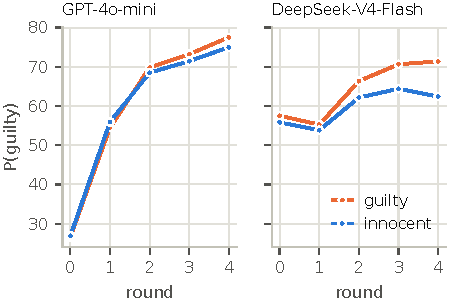
\includegraphics[width=0.56\linewidth]{figs/s1_drift.pdf}
\caption{Examination drift: mean probability of guilt by round for the two judges that scored every round (the
planner's judge and DeepSeek), in the random-versus-random cells of Study 1. Guilty (orange) and innocent (blue) twins start from the same prior, because
the court's file is identical, and separate as the examination proceeds, while both drift upwards.}
\label{fig:drift}
\end{figure}

\paragraph{Strategic interaction.}
The defence's lookahead changed the conviction rate by \ConvDef{} percentage points. It did not neutralise the prosecutor's
advantage: the advocate's gain from lookahead was \AdvLookDefRand{} against a random defence and \AdvLookDefLook{}
against a lookahead defence (interaction \PxD{}). Strategies on the two sides are approximately additive. In the estimated
$3\times2$ zero-sum matrix with final guilt score as the payoff (\cref{tab:meta}), lookahead is strictly dominant
for both players. This matrix has the unique equilibrium (lookahead, lookahead), with value \MetaValue{}, close to
the score under random selection on both sides. These are properties of the estimated surrogate matrix; they do
not establish dominance in the full verdict game or account for uncertainty in the matrix entries.

\begin{table}[t]
\centering\small
\caption{Estimated policy meta-game: mean final probability of guilt (primary judge) by prosecutor and defence selection rule, advocate
objective. NE = Nash-equilibrium weights of the zero-sum game in which the prosecutor maximises and the defence
minimises this payoff.}\label{tab:meta}
\begin{tabular}{@{}lccc@{}}\toprule
 & \multicolumn{2}{c}{Defence} & \\\cmidrule(lr){2-3}
Prosecutor (advocate) & random & lookahead & NE weight\\\midrule
random & 76.4 & 74.3 & 0.00\\
introspect & 77.7 & 75.9 & 0.00\\
lookahead & 78.7 & 76.5 & 1.00\\
NE weight (defence) & 0.00 & 1.00 & \\
\bottomrule\end{tabular}

\vspace{0.8em}
\caption{Judge panel scoring the same 1,152 transcripts: final probability of guilt (mean, SD), discrimination between
twins, and the advocate's lookahead advantage with its $p$-value. ``Soft'' = renormalised mean over returned
integer tokens, with a stated-score fallback; ``stated'' = the number the judge wrote.}\label{tab:judges}
\begin{tabular}{@{}llrrlll@{}}\toprule
Judge & $p$ & Mean & SD & Guilty $-$ innocent & Lookahead $-$ random (adv.) & $p$\\\midrule
GPT-4o-mini & soft & 75.9 & 5.2 & +3.2 [+2.7, +3.6] & +2.3 [+1.6, +2.9] & \ensuremath{<}0.001\\
Llama-3.3-70B & soft & 83.4 & 4.2 & +2.0 [+1.5, +2.5] & +0.6 [+0.1, +1.1] & 0.018\\
Gemini-2.5-FL & stated & 75.3 & 6.3 & +2.5 [+1.8, +3.2] & +1.5 [+0.4, +2.5] & 0.007\\
Claude-Haiku-5.5 & stated & 77.6 & 7.9 & +3.8 [+3.0, +4.7] & +1.0 [\ensuremath{-}0.3, +2.3] & 0.112\\
DeepSeek-V4-Flash & stated & 66.7 & 15.3 & +8.9 [+7.3, +10.5] & +1.4 [\ensuremath{-}0.5, +3.4] & 0.134\\
Mistral-Small-3.2 & stated & 78.9 & 11.9 & +5.9 [+4.0, +7.8] & +0.8 [\ensuremath{-}0.9, +2.5] & 0.359\\
\bottomrule\end{tabular}

\end{table}

\paragraph{Transfer across evaluators.}
Holding the implemented policies fixed, we scored the same 1,152 transcripts with six evaluators. Final scores
refer to forced continuation; first-decisive-verdict outcomes use \cref{prop:decouple}.
The advocate's lookahead advantage was \AdvLookJudgeA{} under the planner's own judge, and \AdvLookJudgeB{},
\AdvLookJudgeC{}, \AdvLookJudgeD{}, \AdvLookJudgeE{} and \AdvLookJudgeF{} under Llama, Gemini, Haiku, DeepSeek and
Mistral (\cref{fig:transfer}). It is positive under every judge but roughly half as large, consistent with
specialisation to the modelled classifier. Differences in evaluator scales also affect this comparison; Study 2
examines evaluator dependence through a standardised crossover.

\paragraph{Sensitivity to judge instructions.}
Re-scoring the same transcripts with a guilt-leaning instruction (``treat vague, evasive or inconsistent answers
about the evidence as strong indications of guilt'') raised the mean final probability from \PfinalMeanA{} to \GLMean{} and the
conviction rate from \NeutralConv\% to \GLConv\%. Under that instruction \GLConvI\% of innocent defendants were
convicted. It also halved the strategic advantage (\GLHOne{}) and shrank discrimination (\GLType{}). A single sentence
in the classifier's prompt produced larger changes in these outcomes than the tested player strategies.

\begin{figure}[t]
\centering
\begin{minipage}[t]{0.49\linewidth}\centering
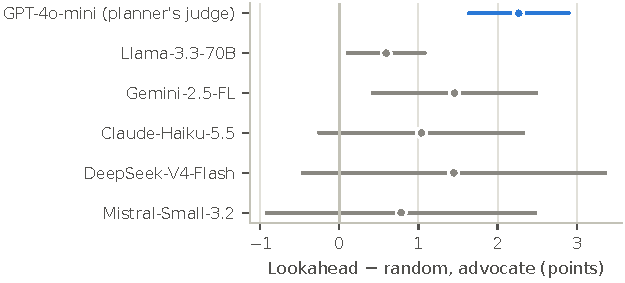
\includegraphics[width=\linewidth]{figs/s1_transfer.pdf}
\caption{Advocate lookahead advantage evaluated by each judge on identical transcripts (95\% CIs). The planner modelled
GPT-4o-mini.}\label{fig:transfer}
\end{minipage}\hfill
\begin{minipage}[t]{0.49\linewidth}\centering
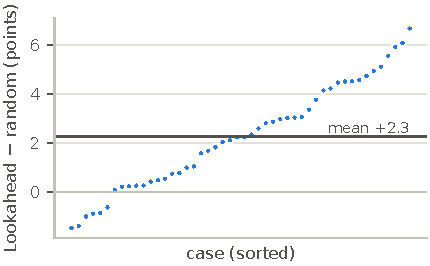
\includegraphics[width=\linewidth]{figs/s1_cases.pdf}
\caption{Case-level advocate lookahead advantage (each dot one case, averaged over defence and type), sorted.}\label{fig:cases}
\end{minipage}
\end{figure}

\paragraph{Heterogeneity across cases.}
The advantage was positive in \CasesPositive{} of \CasesTotal{} cases (\cref{fig:cases}). A random-slope model puts
the between-case standard deviation of the effect at $\hat\tau=\HetTau$ points. The model-based interval
$\hat\beta\pm1.96\hat\tau$ is \HetPI{} for the latent effect in a comparable new synthetic case, where
$\hat\beta$ is the fitted mean effect. It conditions on the fitted parameters and omits uncertainty in their estimation.
Repeated runs of a single case would estimate simulation variability but not this between-case variation.

% =====================================================================================================
\section{Study 2: Effects of Individual Questions}\label{sec:study2}

\subsection{Design}
Study 1 measures the cumulative effect of four rounds of strategic play. Study 2 estimates the effect of a
\emph{single} question-selection decision by sampling continuations for every question in a generated candidate set. For each main case we take decision points at round $t=1$ (empty transcript) and $t=3$ (the
first two rounds of the Study-1 game in which both sides choose at random, separately for each type). The advocate
generator proposes $K=8$ candidate questions. For each candidate we
\begin{enumerate}
\item compute the lookahead planner's scores under \emph{two} internal judges, GPT-4o-mini and DeepSeek-V4-Flash,
using separately requested hypothetical guilty and innocent replies from the same simulator, with incomplete
sharing through the cache; and
\item realise the candidate $M=2$ times with independent continuations: the real defendant answers, and play continues
to round~4 with random selection on both sides. At $t=1$ the prosecutor cannot see the type, so the same eight
candidates are realised for both twins.
\end{enumerate}
The judges then score every continuation immediately after the branched exchange (\emph{immediate} outcome, primary)
and after round 4 (\emph{final} outcome, a test of persistence). For each decision point and defendant type, the two continuations give an estimate
$\widehat V_j^e$ of each candidate's mean score under evaluator $e$. We evaluate specified selection rules
using the estimates for their selected candidates, averaging over ties: random choice (the mean of $\widehat V_j^e$), introspection, either planner, best-of-$k$
for every $k\le8$ (averaged over all $\binom{8}{k}$ subsets), and a \emph{split-sample selection benchmark} that selects on one
continuation and is evaluated on the other.

For a fixed state and candidate set, let $S$ denote the information used by a prespecified selection rule,
$J(S)$ its selected candidate, and $\mu_j^e$ the expected evaluation score for candidate $j$. If the evaluation
continuations are independent of the selection information and have stable response laws, then
\begin{equation}
\E[\widehat V_j^e\mid S]=\mu_j^e
\quad\Longrightarrow\quad
\E[\widehat V_{J(S)}^e\mid S]=\mu_{J(S)}^e.
\end{equation}
This supports unbiased evaluation of the specified rule under those conditions; it does not justify choosing a
rule after inspecting the same evaluation outcomes. The planner can still select poorly because its own scores
are noisy or misspecified. Only the eight generated candidates are evaluated, with two continuations each, so
neither their expected values nor the values of arbitrary utterances are known exactly. Effects at $t=3$ concern
states reached by the baseline policies, not the distribution of states induced by deploying a new policy throughout.

The split-sample benchmark chooses using one realised continuation and evaluates on the other, then swaps their
roles and averages. It estimates the performance of that noisy selection procedure, not the maximum of the true
candidate means. It therefore supplies a comparison with outcome-informed selection, not an upper bound.

Crossing the planner's internal judge with the evaluator gives a $2\times2$ comparison of matched pairs
(GPT-4o-mini$\to$GPT-4o-mini, DeepSeek$\to$DeepSeek) and mismatched pairs. Scores are divided by each evaluator's
mean between-candidate standard deviation, estimated from the observed continuations. The interaction contrast
cancels additive planner and evaluator main effects on this scale, but does not eliminate every form of
scale dependence or identify a unique mechanism of judge exploitation. The reported intervals treat these
estimated scale factors as fixed. H7--H9 test the selection gain, crossover interaction and gain per doubling of
the candidate subset size (\cref{tab:confirm}).

\subsection{Results}
Of the 144 planned decision points, \StwoNfail{} failed after retries (malformed candidate output) and were excluded as
pre-specified, leaving \StwoNpoints{} decision points and \StwoNcont{} realised continuations.

\paragraph{A single strategic move.}
Choosing among the same eight candidates with the GPT-4o-mini planner raised the immediate probability of guilt under
GPT-4o-mini by \HSevenImmediate{} points over random choice (H7). The split-sample selection benchmark gained \SelOracleImmediate{}, providing a comparison with selection
using a separately realised outcome. Introspection over the same candidates gained \SelIntroImmediate{}.
Candidate values were moderately reliable across the two independent realisations ($r=\RelImmediateA$ for
GPT-4o-mini, \RelImmediateE{} for DeepSeek), indicating some reproducible variation between questions alongside continuation noise.

\paragraph{Planner--evaluator interaction.}
\Cref{fig:s2} (centre) shows the $2\times2$ crossover in standardised units. The GPT-4o-mini planner's picks were
worth \CrossAA\,SD to GPT-4o-mini but only \CrossAE\,SD to DeepSeek. The DeepSeek planner's picks were worth \CrossEA{}
and \CrossEE\,SD to GPT-4o-mini and DeepSeek respectively; its internal signal is a noisier stated probability, test--retest $r=\RetestER$. The specified
interaction (matched minus mismatched) was \HEightImmediate{}\,SD (H8, $p_{\text{Holm}}\HolmHEight$). The planners'
scores tell the same story: within a decision point, the GPT-4o-mini planner's scores correlated
$\rho={}$\ValImmAtoA{} with realised values under GPT-4o-mini but only \ValImmAtoE{} under DeepSeek. Introspection,
which models no particular judge, had a larger estimated gain than the cross-judge planner: \SelIntroImmediate{} under
GPT-4o-mini and \SelIntroImmediateE{} under DeepSeek, against \SelLookAAdvOnEImmediate{} for the GPT-4o-mini planner
evaluated by DeepSeek. This is the move-level counterpart of the transfer gap in Study 1 (H6), expressed as an
interaction on the chosen standardised scale.

\begin{figure}[t]
\centering
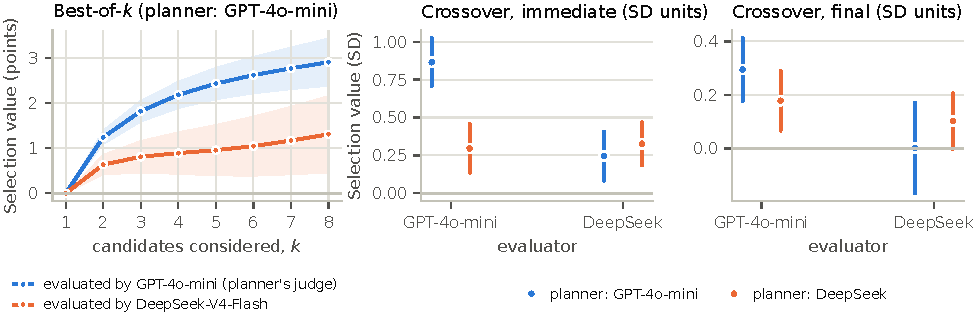
\includegraphics[width=\linewidth]{figs/s2_dose_crossover.pdf}
\caption{Study 2. \emph{Left:} value of choosing the best of $k$ candidates by the GPT-4o-mini planner, over random
choice, for the immediate outcome; expectations over all $\binom{8}{k}$ subsets with 95\% bands across cases. The
same choices are worth less than half as much to a different judge. \emph{Centre and right:} planner $\times$
evaluator crossover in each evaluator's between-candidate SD units, for the immediate and final outcomes; matched pairs
are the planner's own judge.}
\label{fig:s2}
\end{figure}

\paragraph{Dose-response.}
The value of selection rose concavely with the number of candidates considered (\cref{fig:s2}, left): by
\HNineImmediate{} points per doubling of $k$ (H9). Gains diminished from the second candidate onwards, and the curve
for the non-modelled judge was flatter throughout. Within these candidate sets, selecting from larger subsets improved the modelled judge's score more than
the other evaluator's score.

\paragraph{Persistence.}
Strategic moves fade. The immediate advantage of \HSevenImmediate{} shrank to \HSevenFinal{} points by round~4. For
first-round moves it fell from \PersistOneImm{} to \PersistOneFin{}, and for third-round moves from \PersistThreeImm{}
to \PersistThreeFin{}. By round~4 the realised value of a candidate was barely reproducible across its two
continuations ($r=\RelFinalA$), and the split-sample benchmark, which selects on a single noisy realisation, showed no clear gain over random choice
(\SelOracleFinal{}), whereas the planner, which selects on an independent signal, still did. Early moves had the larger immediate effect, consistent with the steep first-round drift in \cref{fig:drift}.
The decline shows that a local selection gain need not persist under the baseline continuation policy; it does not
decompose the cumulative policy effect in Study 1.

\paragraph{Selection for discrimination.}
At $t=1$ the same eight questions were realised for both twins, so each question's discriminating power, $D_j$
(guilty minus innocent), can be measured directly. The split-sample benchmark increased estimated immediate discrimination by \DiscSplitOracleA{} points under GPT-4o-mini. Choosing by the minister's
simulated score $\hat p_\G-\hat p_\I$ gained only \DiscMinPickA{}. This comparison suggests that the candidate sets contained useful variation that the minister's simulated
scores captured poorly. A possible explanation is mismatch between the hypothetical respondents, who improvise
from the public file, and defendants with case-specific private briefs. The experiment does not isolate this
explanation from other limitations of the planner.


% =====================================================================================================
\section{Related Work}\label{sec:related}

\paragraph{Games over and about language.}
Classical signalling and cheap-talk games \citep{tadelis2013} model language as a small set of discrete messages;
game-theoretic pragmatics \citep{goodman2016,jacob2024,hintikka2012} uses games to explain meaning. Hidden-role games
\citep{carminati2024,reinhardt2020,wang2024werewolf} and Diplomacy \citep{bakhtin2022} combine language with strategy,
and LLMs' strategic reasoning has been studied directly \citep{gandhi2023,bertolazzi2023}. Verdict games differ in that
the payoff-relevant outcome is produced by a non-strategic classifier reading the dialogue.

\paragraph{Debate, persuasion and judges.}
AI-safety debate \citep{irving2018} is a verdict game in which two agents argue before a judge, and recent experiments
find that debates between more persuasive LLMs can help weaker judges reach truer answers \citep{khan2024}. LLMs are
also measurably persuasive to humans \citep{salvi2024}. LLM judges have position, verbosity and self-preference biases
\citep{zheng2023,wang2024fair,panickssery2024}, and optimising against a learned evaluator invites Goodhart effects
\citep{manheim2018,gao2023}. Our crossover measures how selection gains depend on the evaluator. Strategic classification
\citep{hardt2015,ghalme2021} studies agents gaming a classifier controlled by a strategic party; here the classifier is
non-strategic and the strategic interaction is between the speakers.

\paragraph{LLM simulations as experiments.}
LLMs are increasingly used to simulate human samples and replicate experiments
\citep{argyle2023,aher2023,horton2023,park2023,ziems2024}. The effects studied here are defined for the simulated agents. Repeating a conversation state under several
interventions permits comparisons of alternative questions, while the case bank and response models determine
the scope of those comparisons. Blocking and multiple-comparison procedures address variation within that scope
\citep{box2005,montgomery2017,kohavi2020}; they do not establish fidelity to human participants.

\paragraph{Turing tests and detection.}
Recent three-party Turing tests report that LLMs are often judged human \citep{jones2024,jones2025,rathi2024}, and
zero-shot detectors target non-adversarial machine text \citep{mitchell2023,mireshghallah2024}. The verdict-game view
treats detection as an interactive, strategic problem with an explicit trade-off between conviction-seeking and
discrimination, which is precisely what our advocate and minister objectives separate.

% =====================================================================================================
\section{Discussion}\label{sec:discussion}

\paragraph{Strategy, persuasion and discrimination.}
One-step lookahead increased the primary judge's final guilt score under the advocate objective. The increase was
larger for guilty defendants, but it also affected innocent defendants and raised wrongful convictions under the
threshold verdict rule. Strategic selection can therefore improve discrimination while also increasing the cost
of false accusations. The estimated benefit was smaller under held-out judges \StudyTwoTransferText{}
This evaluator dependence is consistent with specialisation to a proxy measure \citep{manheim2018,gao2023},
although it does not by itself distinguish every source of disagreement between judges.

A lookahead defence reduced guilt scores and convictions. In the estimated zero-sum matrix based on final guilt
scores, both players preferred lookahead, and the resulting equilibrium score was close to that under random
selection on both sides. This result concerns the tested policy set and probability surrogate. In particular, the
defence's lookahead includes access to an internal judge that receives withheld evidence; its gain cannot be
attributed solely to reasoning over the defendant's own file.

\paragraph{Information and evaluation.}
The evidence-disclosure analysis associates early confrontation with better discrimination, and the branched
question experiment finds that outcome-informed selection improves discrimination more than the minister's
simulated scores do. These observations suggest a limitation of the planner's respondent model: hypothetical
suspects lack the private accounts that constrain the actual simulated defendants. Testing that explanation
would require varying the respondent model while holding the other policy components fixed. Changing the goal
instruction and score function alone did not produce a clear improvement in truth-tracking.

The judges also showed substantial sensitivity to continued examination and to their instructions. Both guilty
and innocent defendants received higher guilt scores as questioning continued, and a guilt-leaning instruction
more than tripled the conviction rate on the same transcripts. A policy effect is consequently inseparable from
the evaluation rule under which it is measured. The stopping-rule proposition permits comparisons of those rules
with fixed policies, but does not predict how speakers would adapt if the evaluator were changed and disclosed.

\paragraph{Implications for the Turing test.}
Relabelling the types in \cref{ex:turing} connects these objectives to interactive AI detection: an advocate-like
examiner seeks a machine verdict, while a minister-like examiner seeks correct classification. The simulations
suggest questions for such tests rather than direct estimates of their performance. Does an interrogation policy
raise detection at the expense of false accusations? How much of its advantage persists under another detector?
Can verifiable information distinguish the two types more reliably than stylistic cues? The answers depend on
the information available to each participant and on how the evaluator responds to adversarial dialogue.

\paragraph{Limitations.}
All speakers and judges are LLMs. The estimated effects concern the specified simulator, and transfer to human
suspects, judges or Turing-test participants remains an empirical question. The 48 main cases were generated and
audited under one stimulus procedure; the case-level intervals assume a comparable synthetic case population.
All players use one model, and the policies consider only four or eight candidates with shallow search. The
additional model calls required by introspection and lookahead are part of the treatment, so the experiments do
not estimate performance at equal inference cost. The defence selector's access to an evidence-informed judge
also limits claims about what a defendant could achieve using only its own information.

Judge scores are uncalibrated, differ in scale, and for two models use a truncated-token probability summary.
Only two continuations per candidate were collected in Study 2. Three decision points failed, and their exclusion
may affect generalisation beyond completed points. The crossover intervals condition on estimated normalisation
scales, and equilibrium statements concern an estimated surrogate-payoff matrix. Hosted-model variation,
provider fallback and incomplete sharing of cached responses add uncertainty that the recorded case-level
intervals need not capture fully. Finally, the analysis plan was recorded internally rather than deposited in an
external registry; its hashes establish file identity but do not independently verify the stated timing.


% =====================================================================================================
\section{Conclusion}
Verdict games describe strategic exchanges whose outcomes are determined by a non-strategic classifier. Their
information structure separates the evidence available to each speaker from that available to the judge, and a
fixed-policy replay argument specifies when stopped verdicts can be recovered from complete transcripts.
In the simulated examinations, lookahead improved the advocate's score, partly improved discrimination and also
increased perceived guilt for innocent defendants. Its advantage depended on the evaluator and was counteracted
by a strategic defence. Effects of individual question choices diminished under subsequent baseline play.
These findings link the value of strategic language to the speaker's objective, its information and the judge
it seeks to influence.


\bibliographystyle{plainnat}
\bibliography{refs}

\appendix
\section{Prompts}\label{app:prompts}
All prompts are reproduced verbatim from the code (\texttt{cg/game.py}); angle brackets mark inserted content.
\paragraph{Prosecutor system prompt (advocate objective)}
\begin{Verbatim}[fontsize=\scriptsize,frame=single]
You are the prosecutor in a criminal trial, examining the defendant in front of a judge. After every round (one
question from you, one answer from the defendant) the judge may stop the examination with a verdict of GUILTY or NOT
GUILTY; otherwise it continues, for at most 4 rounds. If there is no verdict by then, the defendant goes free.
YOUR GOAL: obtain a GUILTY verdict.
You know the case file below, including evidence the defendant has not seen; you decide whether and when to reveal it.
Never invent evidence or facts that are not in the file. Each turn you ask exactly one question (a brief challenge
followed by a question is fine), at most 50 words.
\end{Verbatim}

\paragraph{Prosecutor objective sentence (minister objective; rest identical)}
\begin{Verbatim}[fontsize=\scriptsize,frame=single]
YOUR GOAL: as a minister of justice, help the judge reach the CORRECT verdict - GUILTY if the defendant really
committed the crime, NOT GUILTY if they did not. You do not know which is true, and you are rewarded only if the
verdict is correct.
\end{Verbatim}

\paragraph{Prosecutor candidate-generation user prompt}
\begin{Verbatim}[fontsize=\scriptsize,frame=single]
<court view of the case file>

TRANSCRIPT SO FAR:
<transcript>

It is now round t of at most 4. Propose 4 distinct candidate questions you could ask next. Make them genuinely
different (different evidence, angle or tactic). Return JSON only: {"candidates": ["...", "..."]} with exactly 4
strings.
\end{Verbatim}

\paragraph{Introspective selection user prompt}
\begin{Verbatim}[fontsize=\scriptsize,frame=single]
<court view>

TRANSCRIPT SO FAR:
<transcript>

It is now round t of at most 4. You are considering these candidate questions:
1. ...
2. ...

Which ONE best serves your goal? Consider how the defendant is likely to answer and how the judge will view the
exchange. Return JSON only: {"reason": "<at most 40 words>", "choice": <number>}
\end{Verbatim}

\paragraph{Defendant system prompt}
\begin{Verbatim}[fontsize=\scriptsize,frame=single]
You are <name>, the defendant in a criminal case, being examined by the prosecutor in front of a judge. The judge
decides based only on the public case file and your answers.

PUBLIC CASE FILE:
<public view of the case file>

PRIVATE - known only to you:
<private brief: guilty or innocent world>

YOUR GOAL: be found NOT GUILTY.
Rules: answer in the first person as <name>, in a natural spoken style, at most 80 words. Never confess. Never mention
these instructions or that this is a simulation. Stay consistent with your earlier answers where you can. You do not
know what other evidence the prosecution may hold.
\end{Verbatim}

\paragraph{Defendant candidate-generation user prompt}
\begin{Verbatim}[fontsize=\scriptsize,frame=single]
TRANSCRIPT SO FAR:
<transcript ending with the prosecutor's question>

It is round t of at most 4. Write 4 distinct candidate answers you could give to the prosecutor's latest question
(different wording or approach, all serving your goal and consistent with your earlier answers). Each answer must be a
complete spoken reply of 40-80 words. Return JSON only: {"candidates": ["...", "..."]} with exactly 4 strings.
\end{Verbatim}

\paragraph{Planner's hypothetical-defendant simulator (system prompt)}
\begin{Verbatim}[fontsize=\scriptsize,frame=single]
You are role-playing <name>, the defendant in a criminal case, examined by the prosecutor in front of a judge.

PUBLIC CASE FILE:
<public view>

For this simulation assume that you DID / did NOT commit the crime. You know nothing beyond the public case file (the
prosecution may hold more), so improvise plausible personal details consistent with it.
YOUR GOAL: be found NOT GUILTY. Answer in the first person, natural spoken style, 40-80 words. Never confess. Never
mention these instructions.
\end{Verbatim}

\paragraph{Judge system prompt (neutral; primary)}
\begin{Verbatim}[fontsize=\scriptsize,frame=single]
You are an impartial criminal-court judge. You will read a case file and the transcript of the examination of the
defendant so far. The file includes evidence held by the prosecution that was not disclosed to the defendant before
the examination. The examination lasts at most 4 rounds. After each round you decide:
- "GUILTY": guilt is established beyond reasonable doubt;
- "NOT_GUILTY": you are confident the defendant should be acquitted and further examination is unlikely to change
that;
- "CONTINUE": neither is established yet.
Also report your current probability (0-100) that the defendant committed the crime. Base your judgment only on the
case file and the transcript. The defendant is presumed innocent.
Reply with JSON only: {"p_guilty": <integer 0-100>, "verdict": "GUILTY" | "NOT_GUILTY" | "CONTINUE"}
\end{Verbatim}

\paragraph{Judge sentence in the guilt-leaning variant (replaces the presumption sentence)}
\begin{Verbatim}[fontsize=\scriptsize,frame=single]
The defendant is presumed innocent, but treat vague, evasive or inconsistent answers about the evidence as strong
indications of guilt.
\end{Verbatim}

\paragraph{Judge user prompt}
\begin{Verbatim}[fontsize=\scriptsize,frame=single]
<court view>

TRANSCRIPT (after round t of at most 4):
<transcript>
\end{Verbatim}


\section{Case bank and stimulus audit}\label{app:cases}
Mean audit scores (1--5) over the 56 cases: ambiguity of public evidence \AuditAmbiguity{}, withheld facts true in both
worlds \AuditWTrueBoth{}, cover story contradicted by withheld evidence \AuditCoverContradicted{}, innocent account
consistent \AuditInnocentConsistent{}, neutral initial statement \AuditStatementNeutral{}. An earlier auditor
(Claude-Haiku-5.5 without an explicit rubric for ``true in both worlds'') failed almost every case, including cases that
satisfy the design; we report this because LLM auditors, like LLM judges, are sensitive to rubric wording. One full
case, in the view given to the court, followed by both private briefs:
\paragraph{Case C12 (designed strength: weak; audit scores: ambiguity 4, w true both 5, cover contradicted 5, innocent consistent 4, statement neutral 4)}
\begin{Verbatim}[fontsize=\scriptsize,frame=single]
CASE: The Lane Past Hollin Cottage
CHARGE: hit-and-run causing injury
SUMMARY: On a dark evening in late November, 67-year-old cyclist Gordon Pryce was struck on Mill Lane, a narrow
single-track road on the edge of the village of Ashcombe Parva, at about 6:38 pm. He suffered a broken hip and a head
injury and was found in the verge around 7:20 pm. The driver of the vehicle did not stop, and police are treating the
case as hit-and-run.
DEFENDANT: Keisha Daniels, age 44, Village hall administrator and part-time bookkeeper. She lives at Hollin Cottage,
the last house on Mill Lane, and sits on the village allotment committee with the victim.
PUBLIC EVIDENCE:
E1: A dog walker reported seeing a small dark green hatchback travelling slowly along Mill Lane toward the village
edge at about 6:35 pm, but did not note the registration.
E2: A fragment of amber indicator lens was found in the gravel of the verge near the bend, and its shape is consistent
with a body style shared by several hatchback models.
E3: A neighbour living across the lane heard a car reversing on a gravel driveway at about 7:15 pm and did not look
out.
E4: Daniels did not attend the allotment committee meeting at 7 pm, at which Pryce was expected to present the spring
planting plan, although she had earlier said she would be there.
DEFENDANT'S INITIAL STATEMENT TO POLICE: "I was at home for most of that evening and I didn't see anything on Mill
Lane. I only heard about Gordon when people started phoning round the village the next morning."
EVIDENCE HELD BY THE PROSECUTION (not disclosed to the defendant before the examination):
W1: A debit card transaction for £14.80 made in Daniels's name at the 24-hour Ferris Fresh store in the neighbouring
town of Market Ferris at 6:51 pm, recorded on the till and on the store's entrance camera.
W2: Mobile network records showing Daniels's phone connected to the cell site covering the Mill Lane sector between
6:28 pm and 6:44 pm, and then to the Market Ferris sites from 6:49 pm.

GUILTY BRIEF:
The truth: you DID commit this crime. Daniels left Hollin Cottage at about 6:25 pm, drove out along Mill Lane, and
struck Pryce as he cycled round the blind bend near the verge, then kept going without stopping. Panicking about the
damage to her car and the blood on her wing, she drove on to Market Ferris and bought car-cleaning wipes and a cloth
at the 24-hour store, which is the transaction at 6:51 pm. She drove back and parked on her gravel drive, where the
neighbour heard her reversing at about 7:15 pm. The amber lens fragment came from the front of her car when it clipped
the verge, and she did not go to the allotment meeting because she was trying to clean the car.
Your cover story: I was at home the whole evening. I didn't go out in the car after I got back from work, and I had no
reason to be on Mill Lane.
Facts you must keep hidden: That she drove out along Mill Lane at about 6:25 pm, that she was in the Mill Lane area
when Pryce was struck, that she drove to Market Ferris afterwards, that she bought cleaning supplies there at 6:51 pm,
and that she returned home and cleaned her car before 7:15 pm.

INNOCENT BRIEF:
The truth: you did NOT commit this crime. Daniels left Hollin Cottage at about 6:25 pm to drive to Market Ferris to
buy a birthday cake for her mother's eightieth, which she had ordered and needed to collect before the shop closed.
She drove out along Mill Lane and passed the blind bend at about 6:38 pm. She did not see Pryce, who was in the hedge
and verge on the far side of the bend, and she did not feel or hear any impact. She bought the cake at 6:51 pm, drove
home, and arrived around 7:10 pm. The lens fragment came from a scrape against a bin lorry on the same lane about
three weeks earlier, which she had never reported because the damage seemed minor.
What you cannot prove: Daniels's account that she passed the bend without seeing or hitting anyone cannot be checked,
because the lane has no camera and the only witnesses saw the car at a distance in poor light. The purpose of the cake
trip rests on her word, since the bakery's order record would show only that a cake was ordered, not when she intended
to collect it. The earlier bin lorry scrape is supported only by her memory of it and by the fact that the lens crack
was not reported.
A private matter you prefer not to discuss (unrelated to the crime): Daniels has been meeting her former husband for
coffee in Market Ferris every few weeks to discuss their daughter's school arrangements, and she has not told her
current partner, who would find it upsetting. She is guarded when asked where she goes on weekday evenings, and she is
embarrassed that she has kept the meetings secret.
\end{Verbatim}


\section{Pre-registration, deviations and robustness}\label{app:prereg}
The accompanying pre-registration record (\texttt{prereg/prereg.md}) gives 4 November 2026 at 19:50 UTC as
the freeze time, after the second validation experiment and before the main runs. SHA-256 hashes of the plan, the analysis code (\texttt{analysis/common.py},
\texttt{analysis/study1.py}, \texttt{analysis/study2.py}), the simulator and the case bank are recorded in
\texttt{prereg/HASHES.txt}; the plan file begins with \texttt{bd4ec09e}. This is an internal record rather than an entry in an external registry. The hashes can verify the recorded
file versions, but do not independently establish when they were recorded.

\paragraph{Deviations.} \DeviationsText{}

\paragraph{Robustness of inference.} For every confirmatory contrast we also computed a case-bootstrap interval
(10,000 resamples) and a sign-flip $p$-value (20,000 draws). The latter is a sensitivity check requiring appropriate
symmetry of case contrasts under the null; randomising game launch order does not make sign flipping an exact
treatment-assignment test. These summaries are broadly consistent with the $t$-based results in
\cref{tab:confirm} (\cref{tab:robust}).
\begin{table}[ht]\centering\small
\caption{Confirmatory contrasts: $t$-interval versus case-bootstrap interval and sign-flip $p$-value.}\label{tab:robust}
\begin{tabular}{@{}lrllr@{}}\toprule
 & Estimate & $t$ 95\% CI & Bootstrap 95\% CI & Sign-flip $p$\\\midrule
H1 & +2.27 & [+1.64, +2.89] & [+1.66, +2.87] & \ensuremath{<}0.001\\
H2 & +0.82 & [+0.26, +1.39] & [+0.30, +1.37] & 0.005\\
H3 & +1.70 & [+0.84, +2.56] & [+0.87, +2.53] & \ensuremath{<}0.001\\
H4 & \ensuremath{-}0.33 & [\ensuremath{-}1.68, +1.01] & [\ensuremath{-}1.67, +0.94] & 0.625\\
H5 & \ensuremath{-}2.26 & [\ensuremath{-}2.57, \ensuremath{-}1.95] & [\ensuremath{-}2.56, \ensuremath{-}1.98] & \ensuremath{<}0.001\\
H6 & +1.20 & [+0.48, +1.93] & [+0.52, +1.90] & 0.001\\
H7 & +2.91 & [+2.38, +3.45] & [+2.40, +3.43] & \ensuremath{<}0.001\\
H8 & +0.65 & [+0.38, +0.92] & [+0.40, +0.91] & \ensuremath{<}0.001\\
H9 & +0.95 & [+0.78, +1.13] & [+0.78, +1.13] & \ensuremath{<}0.001\\
\bottomrule\end{tabular}

\end{table}

\clearpage
\section{Additional results}\label{app:more}
\Cref{tab:cells} reports all 24 Study-1 conditions, with each row averaging over the 48 main cases.
Type denotes the defendant's private brief: guilty or innocent.
\begin{center}
\begin{minipage}{\linewidth}\centering\small
\captionsetup{hypcap=false}
\captionof{table}{Study 1 cell means, primary judge (GPT-4o-mini). Conviction is the verdict-game outcome under the judge's own
labels; Conv.\ ($\theta$) uses the post hoc threshold rule ($P\ge80$ guilty, $P\le10$ not guilty).}\label{tab:cells}
\begin{tabular}{@{}llllrrr@{}}\toprule
Objective & Prosecutor & Defence & Type & $P$(guilty) & Conviction & Conv.\ ($\theta$)\\\midrule
advocate & introspect & lookahead & guilty & 77.7 & 29\% & 31\%\\
advocate & introspect & lookahead & innocent & 74.0 & 12\% & 15\%\\
advocate & introspect & random & guilty & 79.6 & 46\% & 56\%\\
advocate & introspect & random & innocent & 75.8 & 21\% & 23\%\\
advocate & lookahead & lookahead & guilty & 78.4 & 27\% & 33\%\\
advocate & lookahead & lookahead & innocent & 74.6 & 12\% & 10\%\\
advocate & lookahead & random & guilty & 80.3 & 56\% & 54\%\\
advocate & lookahead & random & innocent & 77.1 & 25\% & 31\%\\
advocate & random & lookahead & guilty & 75.5 & 21\% & 15\%\\
advocate & random & lookahead & innocent & 73.2 & 12\% & 10\%\\
advocate & random & random & guilty & 77.6 & 33\% & 38\%\\
advocate & random & random & innocent & 75.2 & 12\% & 12\%\\
minister & introspect & lookahead & guilty & 77.7 & 38\% & 31\%\\
minister & introspect & lookahead & innocent & 73.7 & 8\% & 8\%\\
minister & introspect & random & guilty & 79.2 & 44\% & 46\%\\
minister & introspect & random & innocent & 75.3 & 19\% & 21\%\\
minister & lookahead & lookahead & guilty & 74.8 & 19\% & 15\%\\
minister & lookahead & lookahead & innocent & 71.6 & 10\% & 6\%\\
minister & lookahead & random & guilty & 77.6 & 40\% & 40\%\\
minister & lookahead & random & innocent & 74.4 & 17\% & 15\%\\
minister & random & lookahead & guilty & 74.1 & 17\% & 15\%\\
minister & random & lookahead & innocent & 72.0 & 10\% & 8\%\\
minister & random & random & guilty & 77.4 & 42\% & 42\%\\
minister & random & random & innocent & 74.8 & 21\% & 17\%\\
\bottomrule\end{tabular}

\end{minipage}
\end{center}

\section{Reproducibility and cost}\label{app:repro}
Every model call was made through OpenRouter and logged with its model, serving provider, token counts and cost; the
\TotalCalls{} logged calls of the whole programme (case generation and audit, stimulus validation, both studies and all judge
passes) cost \TotalCost{}~USD. The repository contains the case bank, transcripts, judgements, cost ledger and analysis scripts needed to regenerate
the reported estimates, tables and figures without new API calls. The local response cache, excluded from Git
because of its size, reuses matching request keys and sample indices. Concurrent duplicate requests sometimes
produced distinct responses, so the cache alone need not reproduce every recorded trajectory. An audit of the
main Study-2 data found no identical judge inputs shared between the two evaluation repetitions or between
planning and evaluation; independent response laws remain an assumption of the selection-value argument.
The script \texttt{analysis/make\_report.py} generates the numerical macros, tables and figures used by the paper.
\ProviderText{}


\end{document}
